\documentclass[12pt,]{article}
\usepackage{graphicx}
\usepackage{tikz}
\usetikzlibrary{shapes.geometric, arrows}
\usepackage{amssymb}

\title{Sprawozadanie lernicng}
\author{Tymon Łazowy}
\date{123,2123,12}


\tikzstyle{startstop} = [ellipse, rounded corners, minimum width=2cm, minimum height=1cm,text centered, draw=black,thick,fill=red!0]

\tikzstyle{io} = [trapezium,
trapezium stretches=true,
trapezium left angle=70,
trapezium right angle=110,
thick,minimum width=2cm,
minimum height=0.85cm,
text centered,
draw=black,
fill=blue!0]

\tikzstyle{process} = [rectangle,
minimum width=3cm,
minimum height=0.85cm,
text centered,
text width=3cm,draw=black,thick,fill=orange!0]

\tikzstyle{decision} = [diamond,minimum width=1cm, minimum height=1cm, text centered, draw=black, fill=green!0,thick]

\tikzstyle{arrow} = [thick,->,>=stealth]

\begin{document}
D: brak

S: brak
\begin{figure}[h]
    \centering  
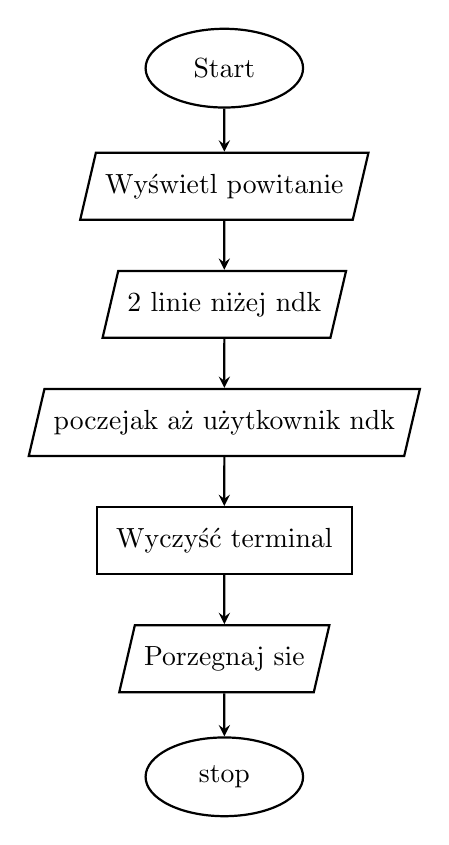
\begin{tikzpicture}[node distance=1.5cm]

\node (start) [startstop] {Start};
\node (out1) [io, below of=start] {Wyświetl powitanie};
\node (out2) [io, below of=out1] {2 linie niżej ndk};
\node (in1) [io, below of=out2] {poczejak aż użytkownik ndk};
\node (pro1) [process, below of=in1] {Wyczyść terminal};
\node (out3) [io, below of=pro1] {Porzegnaj sie};
\node (stop) [startstop, below of =out3]{stop};

\draw [arrow] (start) -- (out1);
\draw [arrow] (out1) -- (out2);
\draw [arrow] (out2) -- (in1);
\draw [arrow] (in1) -- (pro1);
\draw [arrow] (pro1) -- (out3);
\draw [arrow] (out3) -- (stop);


\end{tikzpicture}
    \caption{1.0 flowchart}
    \label{flow2}
\end{figure}
\end{document}